\chapter{Výsledky}\label{chap:results}

Náš model sme testovali na počítači s procesorom Intel\textsuperscript{\textregistered}Core\texttrademark i7-3537U 2.00GHz a grafickou kartou AMD Radeon HD 8670M.

\noindent
V nasledujúcej tabuľke sú merania simulácie nášho modelu pri použití knižnice TNT \cite{tnt}, ktorá používala na riešenie systému lineárnych rovníc tzv. Choleského dekompozíciu. V prvom stĺpci je počet bublín, druhý stĺpec indikuje, či bola pri simulácii zapnutá aj vizualizácia a tretí stĺpec ukazuje počet snímkov za sekundu.

\begin{table}[H]
	\caption{Tabuľka meraní simulácie pri použití knižnice TNT \cite{tnt} s metódou Choleského dekompozície.}
	\setlength{\extrarowheight}{2pt}
	\begin{tabularx}{\textwidth}{|X|X|X|X|}
		\hline
		\textbf{\# bublín} & \textbf{vizualizácia} & \textbf{FPS} \\ \hline
		1         & áno                   & 238          \\ \hline
		5         & áno                   & 115          \\ \hline
		10        & áno                   & 70          \\ \hline
		15        & áno                   & 65           \\ \hline
		15        & nie                   & 150          \\ \hline
		30        & áno                   & 42           \\ \hline
		30        & nie                   & 48           \\ \hline
		50        & áno                   & 12           \\ \hline
		50        & nie                   & 13           \\ \hline
		60        & áno                   & 8            \\ \hline
		60        & nie                   & 8            \\ \hline
		100       & áno                   & 2            \\ \hline
		100       & nie                   & 2            \\ \hline
		120       & áno                   & 2            \\ \hline
		120       & nie                   & 2            \\ \hline
		150       & áno                   & 1            \\ \hline
		150       & nie                   & 1            \\ \hline
	\end{tabularx}
\end{table}

\noindent
Tabuľka \reference{table:viennacl_measurement} obsahuje merania simulácie nášho modelu pri použití knižnice ViennaCL \cite{viennacl} s použitím metódy združených gradientov na riešenie systému lineárnych rovníc. V prvom stĺpci je počet bublín, druhý stĺpec indikuje, či bola pri simulácii zapnutá aj vizualizácia a tretí stĺpec ukazuje počet snímkov za sekundu.

\begin{table}[H]
	\caption{Tabuľka meraní simulácie pri použití knižnice ViennaCL \cite{viennacl} s metódou združených gradientov počítanou na GPU.}
	\label{table:viennacl_measurement}
	\setlength{\extrarowheight}{2pt}
	\begin{tabularx}{\textwidth}{|X|X|X|X|}
		\hline
		\textbf{\# bublín} & \textbf{vizualizácia} & \textbf{FPS} \\ \hline
		1         & áno                   & 227          \\ \hline
		5         & áno                   & 70          \\ \hline
		10        & áno                   & 70          \\ \hline
		15        & áno                   & 68           \\ \hline
		15        & nie                   & 145          \\ \hline
		30        & áno                   & 56           \\ \hline
		30        & nie                   & 70           \\ \hline
		50        & áno                   & 23           \\ \hline
		50        & nie                   & 28           \\ \hline
		60        & áno                   & 18           \\ \hline
		60        & nie                   & 22           \\ \hline
		100       & áno                   & 8            \\ \hline
		100       & nie                   & 9            \\ \hline
		120       & áno                   & 6            \\ \hline
		120       & nie                   & 7            \\ \hline
		150       & áno                   & 4            \\ \hline
		150       & nie                   & 4            \\ \hline
		180       & áno                   & 1            \\ \hline
		180       & nie                   & 1            \\ \hline
	\end{tabularx}
\end{table}

\noindent Z nameraných výsledkov vidieť, že pri menšom množstve bublín bola prvá knižnica využívajúca Choleského dekompozíciu rýchlejšia oproti knižnici využívajúcej metódu združených gradientov a GPU. Toto môže byť spôsobené tým, že sa dáta musia posielať na grafickú kartu. Pri väčšom počte bublín však už vidieť, že druhá knižnica počíta systém lineárnych častíc oveľa rýchlejšie a zatiaľ čo prvá knižnica pri 60 bublinách dokázala simulovať penu pri 8 fps, druhá knižnica pri cca. 8 fps dokázala simulovať 100 až 120 bublín. Výsledky nášho modelu sú pre nás celkom uspokojujúce, aj keď vedeli by sme si predstaviť ešte o niečo väčší počet bublín, ktorý by bol schopný náš model simulovať v reálnom čase.  

\section{Výsledné animácie}

Na obrázku \reference{img:bubble_show_1} vidno 4 podobrázky zobrazujúce animáciu tzv. "Bubble Show". V ľavom hornom podobrázku je vidieť prvú bublinu pridanú do tejto formácie. Na pravom hornom podobrázku vidieť zoskupenie dvoch bublín tejto formácie. Na podobrázku v ľavom dolnom rohu už vidieť 6 bublín tejto formácie. Na poslednom podobrázku v pravom dolnom rohu vidieť výslednú formáciu, kedy je do stredu týchto bublín pridaná posledná bublina obsahujúca dym, ktorá je v tvare kocky, čo je spôsobené vplyvom okolitých bublín, ktoré ju deformujú.
\begin{figure}[H]
	\begin{center}
		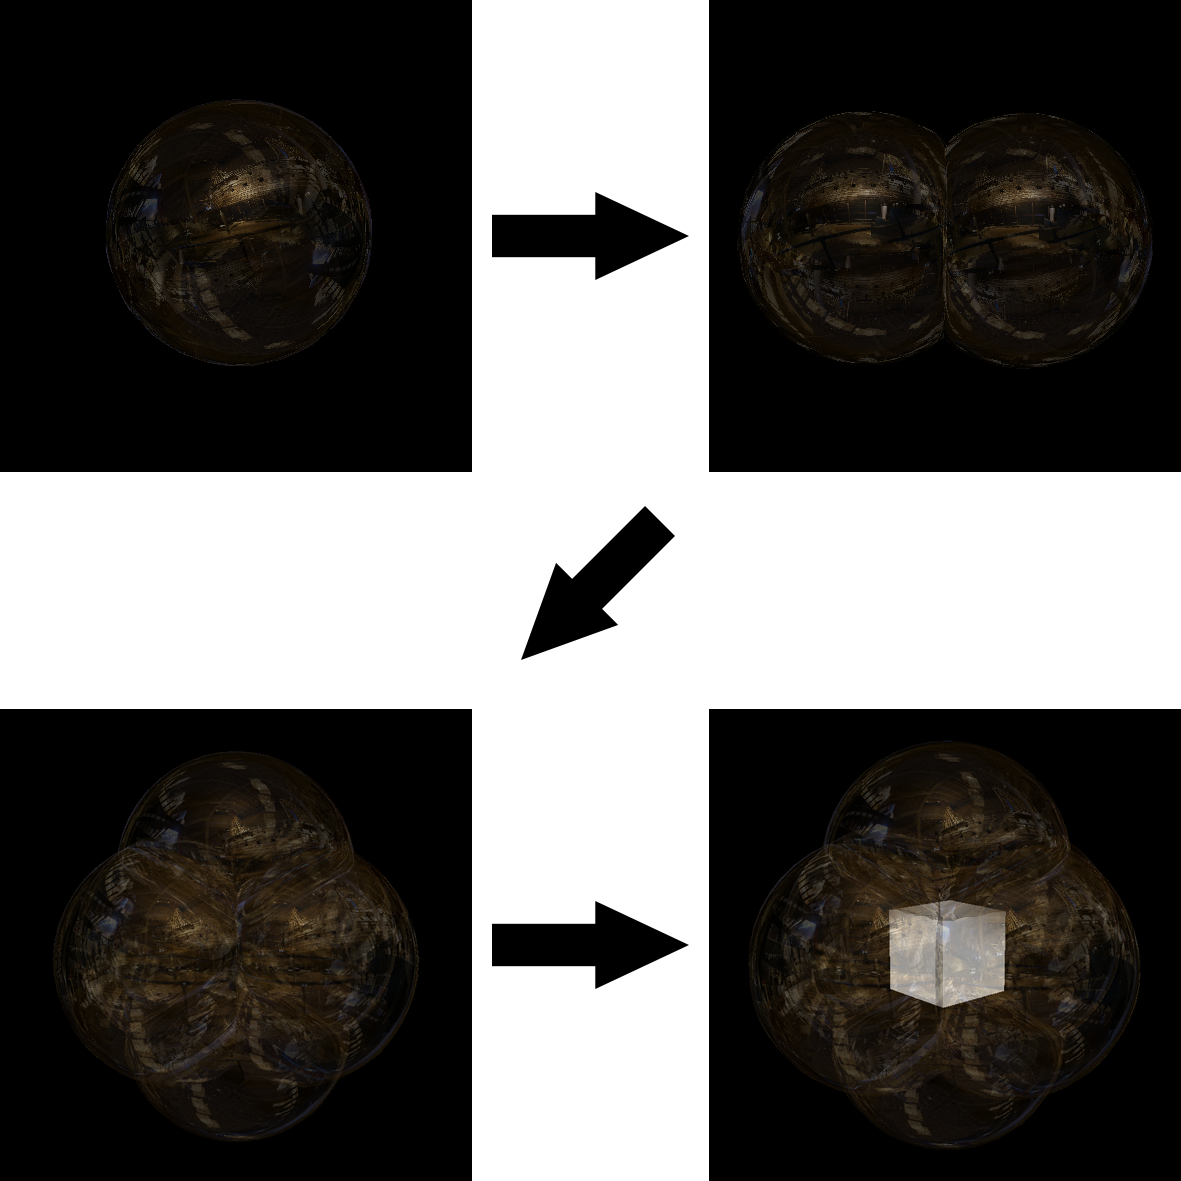
\includegraphics[width=\textwidth]{images/bubble_show_1}
		\caption{Animácia tzv. "Bubble Show" vytvárajúcej kocku uprostred bublín.}
		\label{img:bubble_show_1}
	\end{center}
\end{figure}

Na obrázku \reference{img:bubble_show_2} vidno tiež animáciu zobrazujúcu "Bubble Show". V ľavom hornom podobrázku je opäť vidieť prvú bublinu pridanú do tejto formácie. Na pravom hornom podobrázku vidieť zoskupenie dvoch bublín tejto formácie. Na podobrázku v ľavom dolnom rohu už vidieť 8 bublín tejto formácie. Na poslednom podobrázku v pravom dolnom rohu vidieť výslednú formáciu, kedy je do stredu týchto bublín pridaná posledná bublina obsahujúca dym, ktorá je v tvare šesťbokého hranolu, čo je spôsobené vplyvom okolitých bublín, ktoré ju deformujú.
\begin{figure}[H]
	\begin{center}
		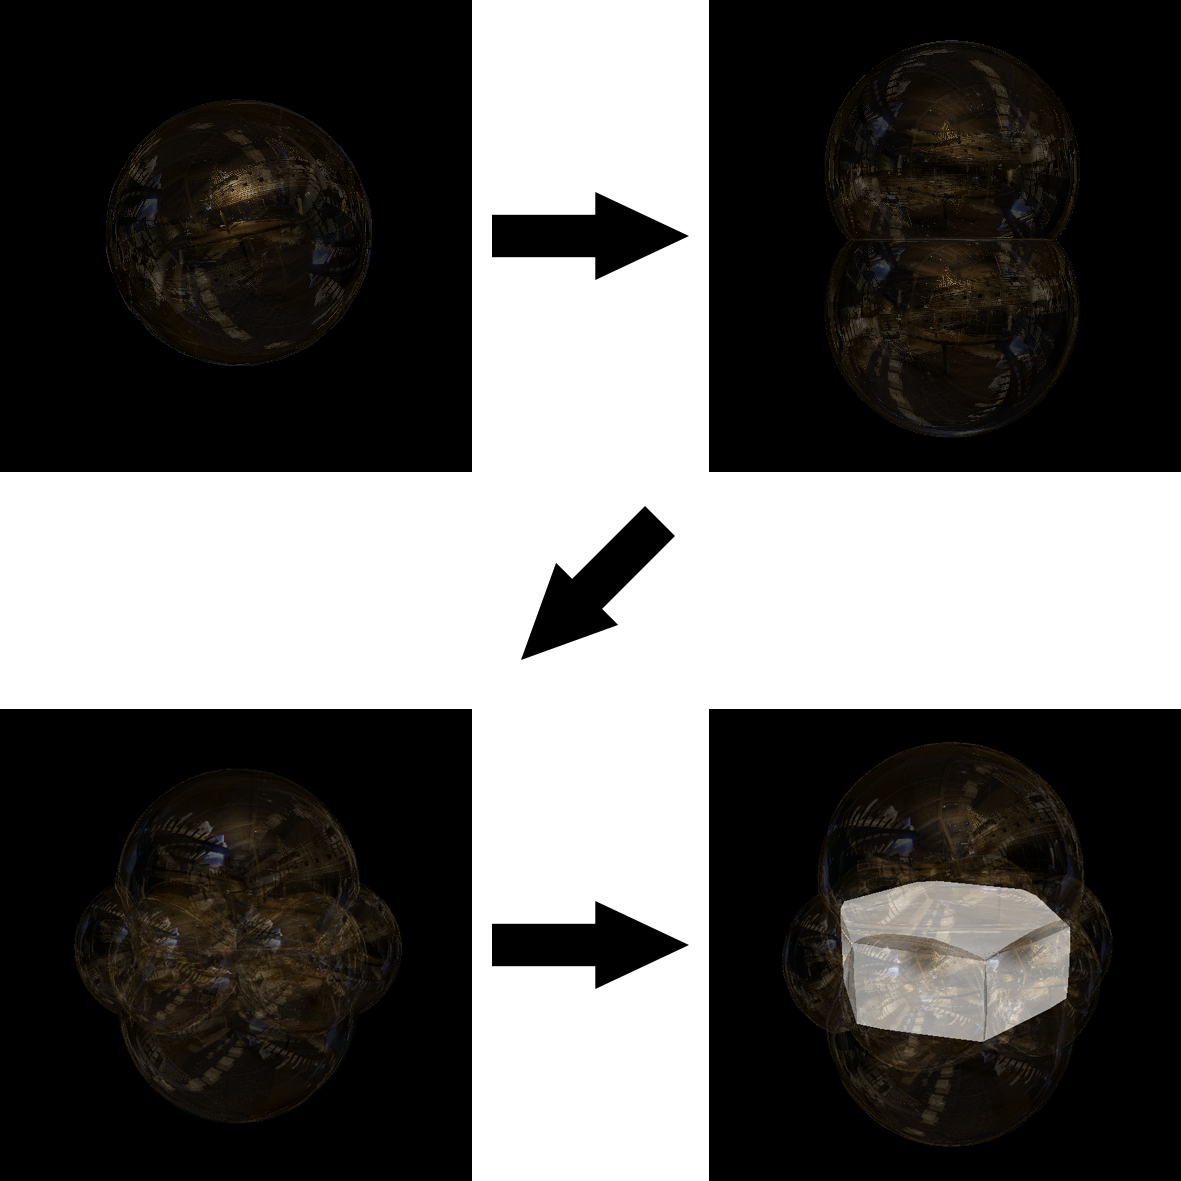
\includegraphics[width=\textwidth]{images/bubble_show_2}
		\caption{Animácia tzv. "Bubble Show" vytvárajúcej šesťboký hranol uprostred bublín.}
		\label{img:bubble_show_2}
	\end{center}
\end{figure}
\newpage
Na obrázku \reference{img:30-bubbles-foam} vidieť penu pozostávajúcu z 30-tich bublín.
\begin{figure}[H]
	\begin{center}
		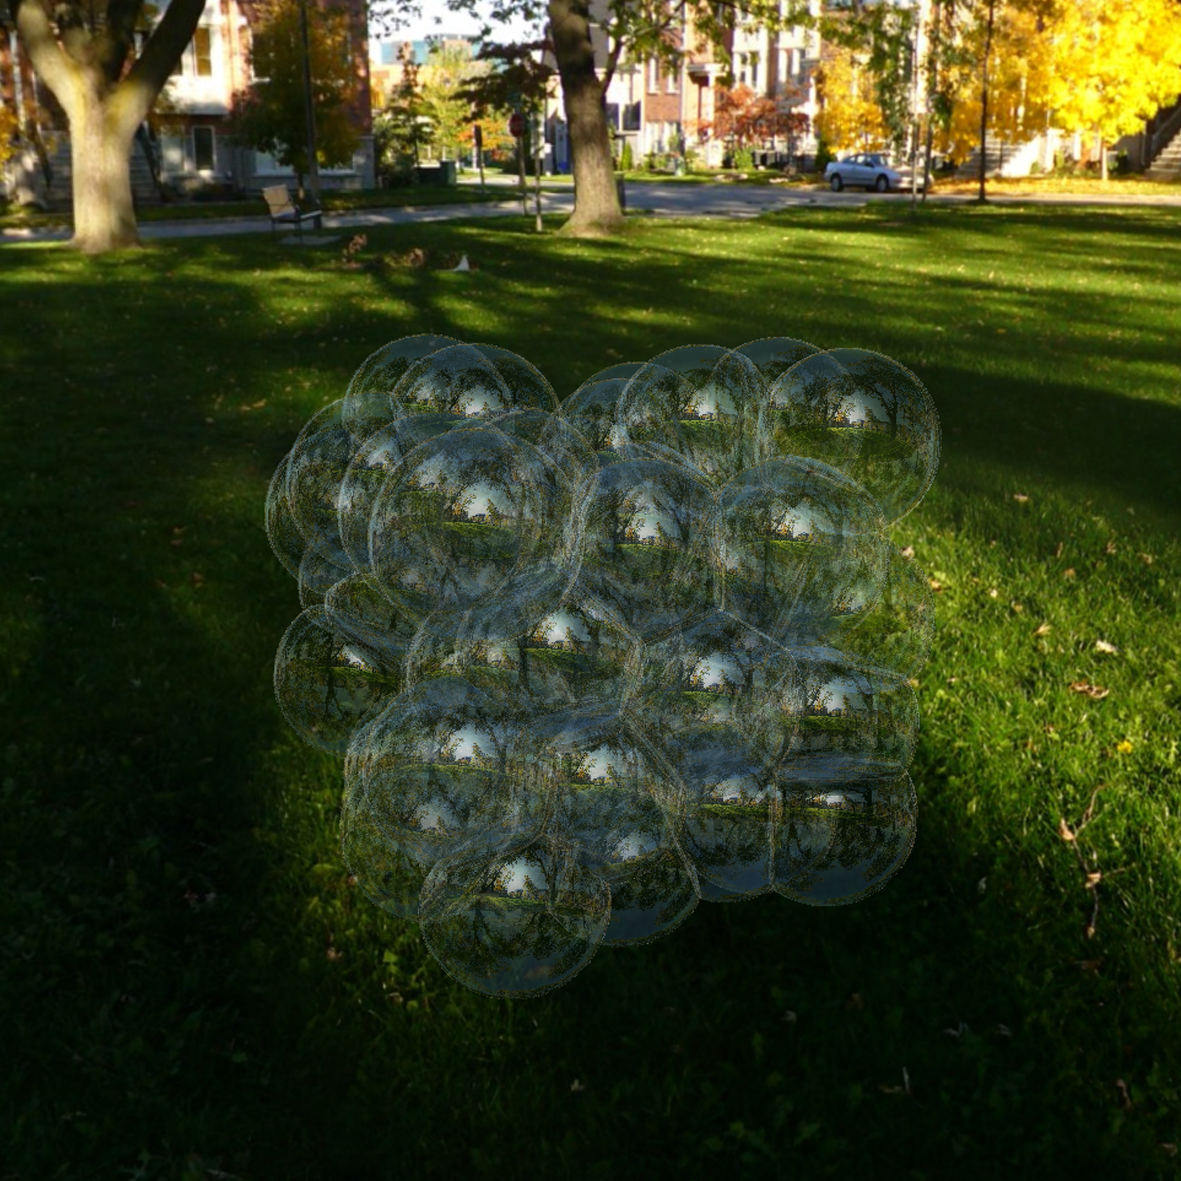
\includegraphics[width=\textwidth]{images/30-bubbles}
		\caption{Pena pozostávajúca z 30-tich bublín.}
		\label{img:30-bubbles-foam}
	\end{center}
\end{figure}
\newpage
Na obrázku \reference{img:120-bubbles-foam} vidieť penu pozostávajúcu zo 120-tich bublín.
\begin{figure}[H]
	\begin{center}
		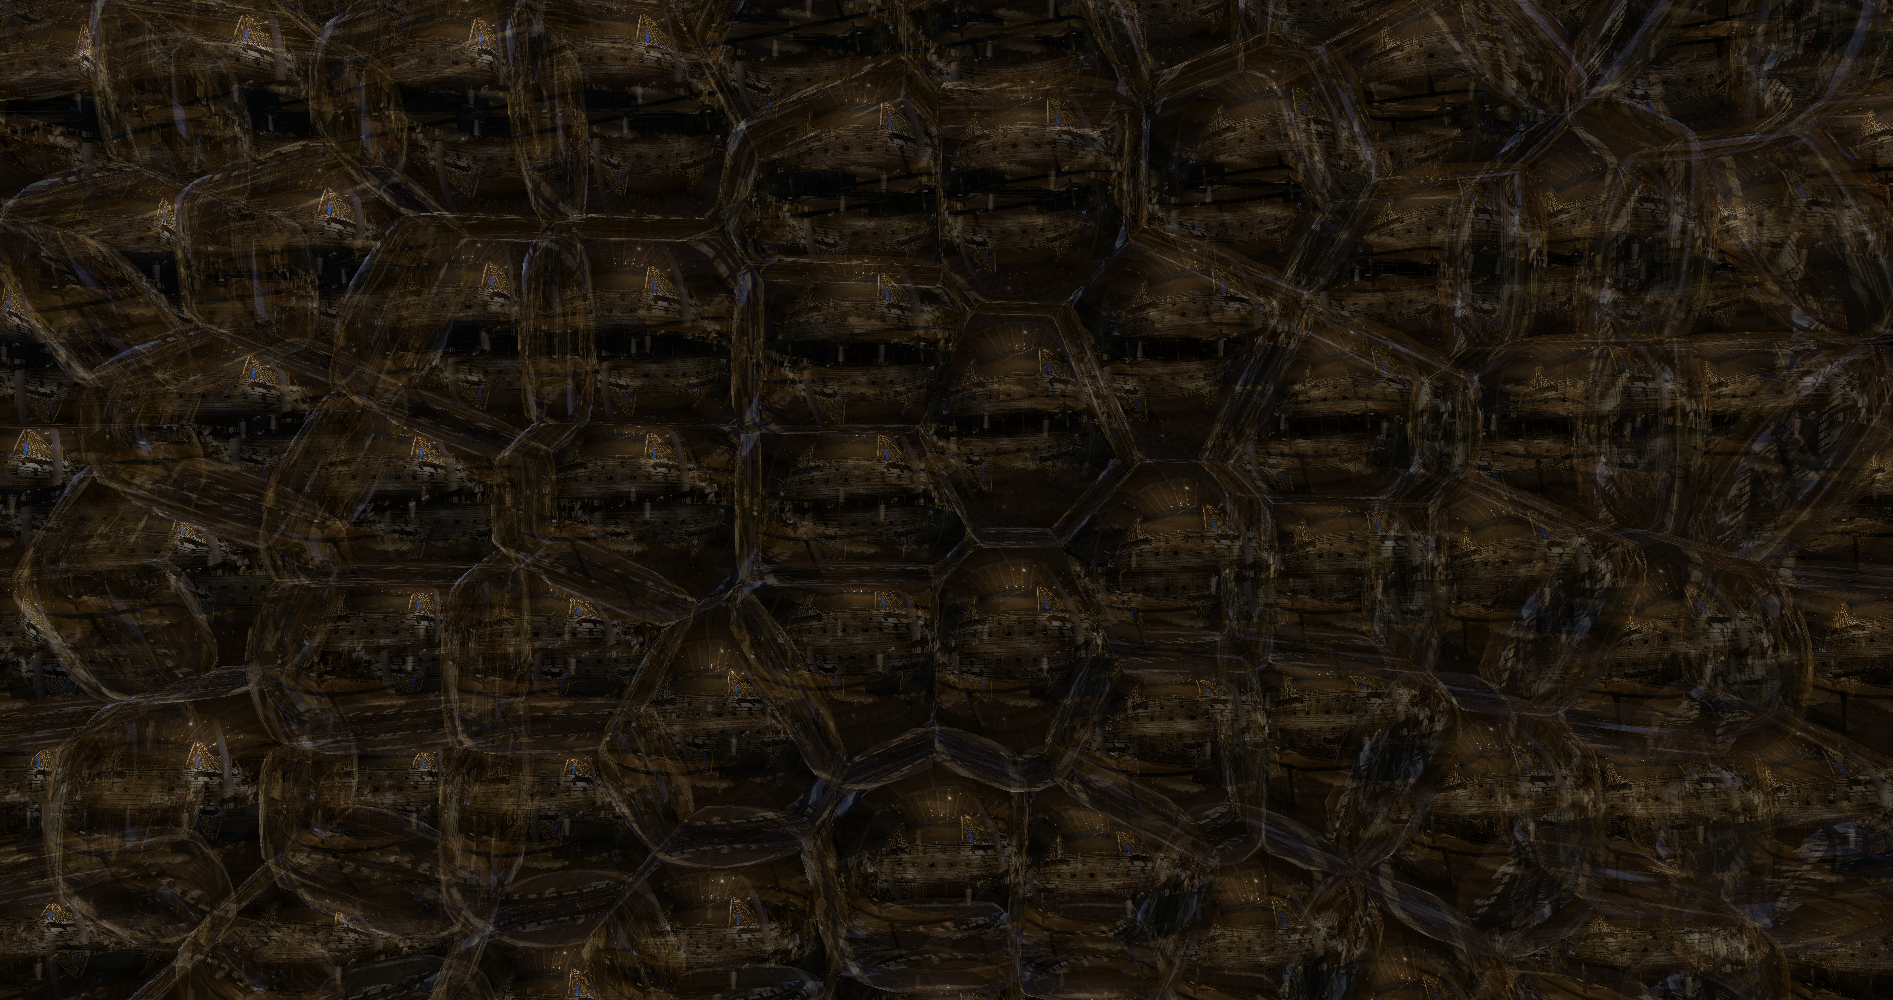
\includegraphics[width=\textwidth]{images/120-bubbles}
		\caption{Pena pozostávajúca zo 120-tich bublín.}
		\label{img:120-bubbles-foam}
	\end{center}
\end{figure}
\newpage
Na obrázku \reference{img:two-bubbles} vidieť detailné zoskupenie dvoch bublín ako aj ich drôtené zobrazenie.
\begin{figure}[H]
	\begin{center}
		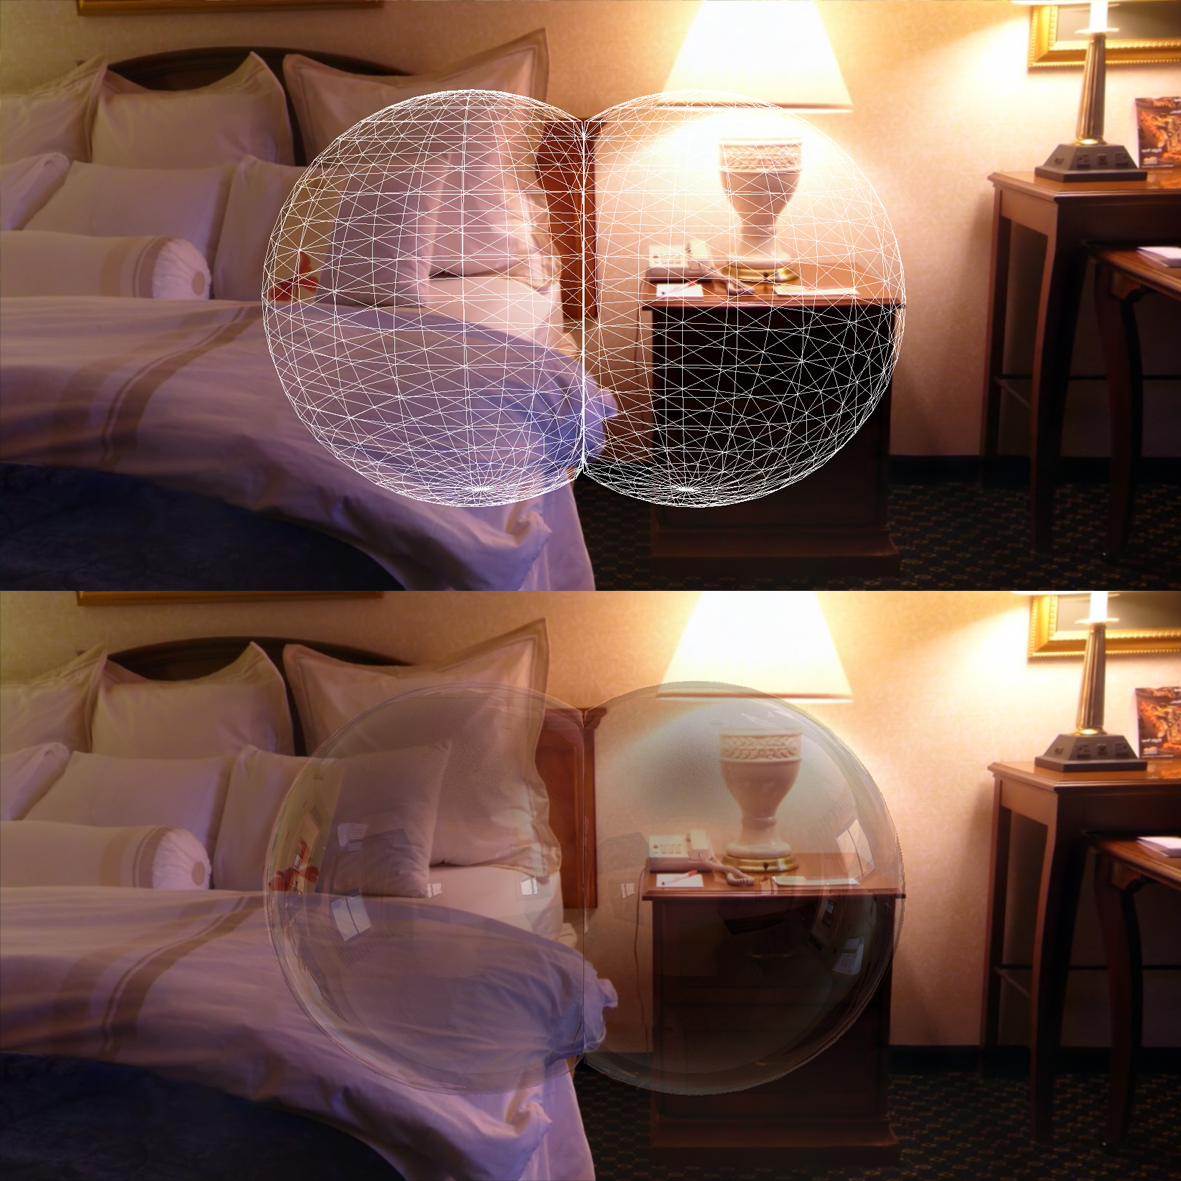
\includegraphics[width=\textwidth]{images/double_bubble}
		\caption{Priesečník dvoch bublín.}
		\label{img:two-bubbles}
	\end{center}
\end{figure}